\documentclass[../main/thesis_msc.tex]{subfiles}

\begin{document}

    \chapter{Introduction}

    Welcome to your thesis template! To begin with, a brief explanation on how to use the template. The main \TeX\, file is \texttt{thesis\_msc.tex} and it is the one that you should be able to compile always. The rest of the files are gathered in subdirectories, and you can compile them independently (with exception of the references). This independent compilation is a good tool, since you'll be adding a ton of text it is a pain to always wait for the \texttt{thesis\_msc.tex} file to finish compiling. By adding small files to compile you have a better and cleaner view of your thesis chapters.



    \section{Citations}
    The citations are same as the ones used in the Astronomy \& Astrophysics Journal (\url{https://www.aanda.org/component/content?view=article&id=160}). Just make sure that your citations are in the same format as the \texttt{bibfile\_thesis.bib}. Finally, after you add a reference you have to compile the pdflatex once, then compile bibtex and compile pdflatex twice, if not you won't see any changes in your pdf file. \\

    \noindent Some in-line citations:
    \begin{itemize}
        \item \citep{bracewell1978fourier}
        \item \citet{bracewell1978fourier}
        \item \citep[see][]{bracewell1978fourier}
    \end{itemize}

    Once you have added the citation in the \texttt{bibfile\_thesis.bib} this will not appear in the reference section, unless it is called with the \texttt{citep\{...\}} command. References won't show up when you compile chapters individually, they will only appear once you compile the \texttt{thesis\_msc.tex} file.

    \section{Notes}
    You can also make nice notes inside your document! Just use the \texttt{note} environment.

    \begin{note}
        You can also change the environment color, add another table shape and other cool things!, go visit the package manual for more information.
        Package manual: \url{https://ctan.org/pkg/tcolorbox?lang=en}.
    \end{note}

    \section{Tables}
    To make nice tables I preferably use the package \texttt{booktabs} (as shown in Table \ref{tab:my_table}), already included. This lets you add bar lines and make the tables more compact. Since it is a matter of taste be free into look some other options.

    \begin{table}[t]
        \centering
        \begin{tabular}{ccc}
            \toprule
            \textbf{A} & \textbf{B} & \textbf{C} \\ \midrule
            1 & 2 & 3 \\
            1 & 2 & 3 \\
            1 & 2 & 3 \\
            1 & 2 & 3 \\
            1 & 2 & 3 \\
            \bottomrule
        \end{tabular}
        \caption{Adding a caption}
        \label{tab:my_table}
    \end{table}

    \section{Tikz figures}
    Tikz (PGF plots) is a powerful tool to create in-line-figures in \LaTeX. Unfortunately requires a lot of time to learn and to be fast adding coordinate systems. There are several examples on-line that you can browse and edit. Making your own figures will always have an extra value in your thesis. There are several sources to learn ho to use Tikz, there are some of them,

    \begin{itemize}
        \item The Tikz package manual, it is long and sometimes misleading but if you want to master Tikz is the right place to start!
        \url{https://www.ctan.org/pkg/pgf}
        \item Several cool examples: \url{http://www.texample.net/}.
        \item Brief introduction: \url{https://www.sharelatex.com/learn/TikZ_package}
    \end{itemize}

    With some command lines you can make something like in Figure \ref{fig:my_fig}.

    \begin{figure}[h]
        \centering
        \begin{tikzpicture}

            \def\linethick{0.6pt}

            \coordinate (M1) at (-2, 0);
            \coordinate (m) at (2, 4);
            \coordinate (M2) at (4, 0);

            \draw[->] (-3, 0) -- (5, 0) node[left, below] {$x$};
            \draw[->] (0, -1) -- (0, 5) node[right] {$y$};

            \draw[line width=\linethick] (0, 0) -- node[midway,left] {$r$} (m) node[above] {$m$};
            \draw[line width=\linethick] (M1) node[above, xshift=-10] {$M_1$} -- node[midway,left] {$s_1$} (m);
            \draw[line width=\linethick] (M2) node[above, xshift=7] {$M_2$} -- node[midway,left] {$s_2$} (m);

            \path (M1) -- node[midway, below] {$r_1$} (0, 0);
            \path (0, 0) -- node[midway, below] {$r_2$} (M2);

            % Dashed lines
            \draw[dashed] (M1) -- ++ (0, -1);
            \draw[dashed] (M2) -- ++ (0, -1);

            \draw[|<->|] ($(M1) + (0, -1.1)$) -- node[midway,fill=white] {$a$} ($(M2) + (0, -1.1)$);

            \node[below] at (0.4, 0) {CM};

            \draw ([shift={(0, 0)}]64:0.5) arc[radius=0.5, start angle=64, end angle=0] node[above, xshift=4] {$\theta$};

            % balck circles
            \filldraw[black] (m) circle(0.1);
            \filldraw[black] (M1) circle(0.17);
            \filldraw[black] (M2) circle(0.13);
            \filldraw[black] (0, 0) circle(0.05);

        \end{tikzpicture}
        \caption{Nice diagram using Tikz.}
        \label{fig:my_fig}
    \end{figure}

    \section{Figures}
    At the time to make the figures, I strongly advice you that use the page width of your \LaTeX file as the default width in your image. This can be easily done by using the \texttt{printlen} package. Then go to your plot routine (e.g.\, Python, \texttt{figsize=(width, height)}) and add the corresponding width. If you have done this correctly you will not have problems in scaling figures in your \TeX\, file.

    \subsection{Figure example}
    Let's create a figure in Python using the correct width of the document. Simply type $\text{width}=\uselengthunit{in}\printlength{\textwidth}$. This width now has to be used in the Python script (see \texttt{figure\_example.py}). Then just import the figure, but without scaling it!

    \begin{figure}[t]
        \centering
        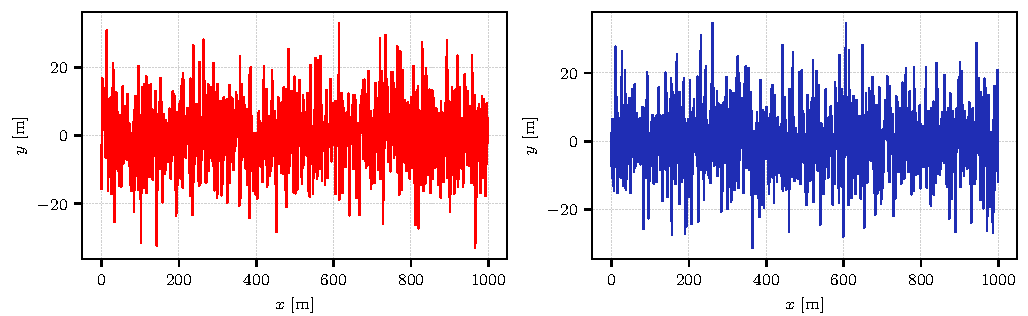
\includegraphics{figure_example.pdf}
        \caption[Adding a figure using Python]{This figure has been created in Python and imported without any scaling (\texttt{includegraphics[scale=0]}). Notice that the text size also matches with the one in this caption, e.g.\ $x$ [m].}
    \end{figure}


\end{document}
